\documentclass[a4paper,10pt]{scrartcl}
\usepackage{physik-vorlesung}

\title{Experimentalphysik I}

\begin{document}

\maketitle

\tableofcontents

\newpage

\section*{Vorwort}
\begin{seg}{Ziele:}
\begin{itemize}
\item Experimentelle und theoretische Grundlagen der Newtonschen Mechanik, Wärmelehre, Thermodynamik
\item Als Einstieg möglichst auf sehr formale u. aufwendige Herleitungen verzichten, Grundprinzipien der Physik verdeutlichen
\item Veranschaulichung des Stoffs durch Demonstrationsexperimente in der Vorlesung
\item An physikalischen Beispielen werden die notwendige Bedingungen geklärt
\end{itemize}
\end{seg}

\begin{seg}{Ist Physik immer streng vorhersehbar?}
häufig ja, aber es gibt auch Ausnahmen:
\begin{itemize}
\item Wettervorhersage
\item \emph{chaotisches Pendel}
\item \emph{Galton-Brett}
\begin{figure}[h]
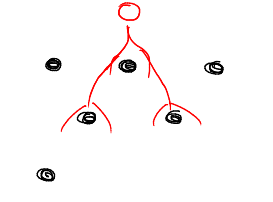
\includegraphics{fig1.png}
\end{figure}
\item \emph{Brownsche Bewegung}

\begin{figure}[h]
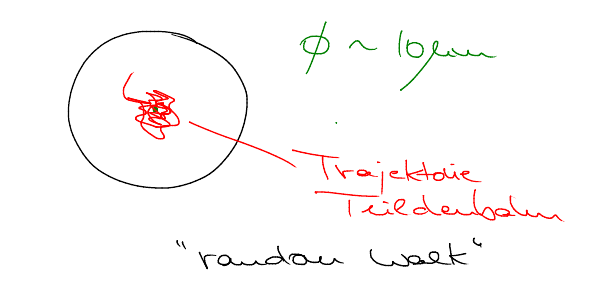
\includegraphics[scale=0.5]{fig2.png}
\end{figure}

\item \emph{Quantenmechanik}\\
Es gilt die Heisenbergsche Unschärferelation:
\[
\underbrace{\Delta x}_{\text{Ortsunschärfe}} \cdot \underbrace{\Delta p}_{\text{Impulsunschärfe}}
\]
\begin{figure}[h]
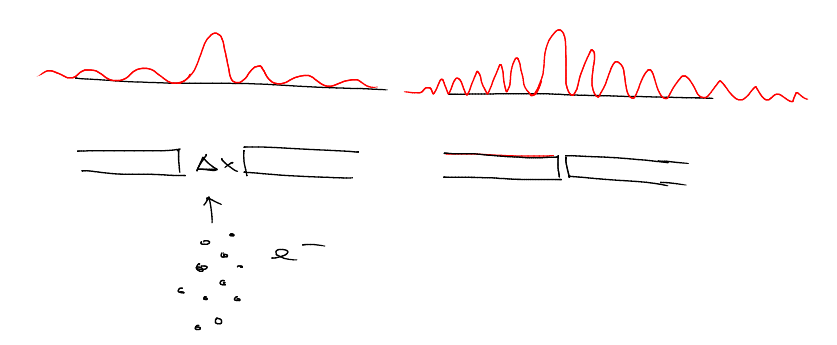
\includegraphics[scale=0.5]{fig3.png}
\end{figure}
\end{itemize}
\section{Physikalische Größen}
Eine \emph{Physikalische Größe} besteht aus einem \emph{Zahlenwert} und einer \emph{Einheit}.
\begin{ex*}
$1 \text{ in } \hat = \text{ Breite d. Daumens}$\\
Dies wurde später dann modifiziert, sodass die Einheit zur Länge drei aneinander liegenden Gerstenkörner umdefiniert worden ist.
\begin{figure}[h]
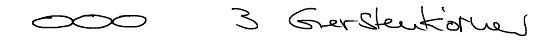
\includegraphics[scale=0.5]{fig4.png}
 \end{figure}
 
 Wünsche: wenige, aber überall nachprüfbare Einheiten $\rightarrow$ Basiseinheiten, Grundeinheiten
 \end{ex*}
 \end{seg}
 \subsection{Basiseinheiten}
 \begin{enumerate}[a)]
\item Zeit \\
Die Grundeinheit der Zeit ist $1$ Sekunde(s).  Diese lässt sich definieren durch den Vergleich mit periodischen Vorgang. Es gilt:
\[
\boxed{T=2\pi \sqrt{\frac{l}{g}}}
\]

\[
l=24,8 \text{cm} \rightarrow T=1s
\]
\begin{itemize}
\item Quarzplättchen besitzen eine Frequenz aus dem $kHz$-Bereich.
\begin{figure}[h]
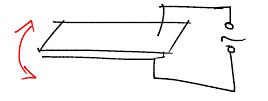
\includegraphics[scale=0.5]{fig5.png}
\end{figure}

Sie Besitzen einen Gangungenauigkeit von $1$ s/Woche. Sie besitzen also einen Fehler von $1$s pro $10^6$s
\item Es gibt aber auch die Möglichkeit mittels atomarer Eigenschwingungen (atomare Uhren) die Zeit noch genauer zu messen.  Deren Ganggenauigkeit entspricht $1$ s/$3000$ Jahren. Dies findet unter anderem Anwendung im GPS. 
\item $\ce{^{133}Cs}$ Hyperfeinübergang

Es ergibt sich die Definition $1\s=9.192.631.770$-faches der Periodendauer des Hyperfeinübergangs in $\ce{^{133}Cs}$. Diese ist überall nachvollziehbar!
\newpage
 \begin{seg}{Größenordungen von Zeiten}
 
 \begin{center}
% \begin{table}[h]
 \begin{tabular}{l r}
 Weltall: & $10^8 \s$ \\
 Mensch: & 1$10^9 s$ \\
 Pulsschlag: & $1 s$ \\
 Licht durchläuft $30 cm$: & $10^-9 s$ \\
 Licht durchläuft Atom: & $10^-18 s$
 \end{tabular}
% \end{table}
 \end{center}
 \end{seg} 
Mit Hilfe von Präfixen kann man den Einheit eine neue Größenordnung geben. Hier die geläufigen Präfixe:

\begin{center}
% \begin{table}[h]
 \begin{tabular}{l c r}
  $1\m$ & Milli & $10^{-3}$\\
  $1\my$ & Mikro & $ 10^{-6}$\\
 $1\n$ & Nano & $ 10^{-9}$ \\
 $1\p$ & Piko & $ 10^{-12}$\\
 $1\f$ & Fakto & $10^{-15}$\\
 $1\a$ & Atte & $10^{-18}$\\
 $1\k$ & Kilo & $10^3$ \\
 $1\M$ & Mega & $10^6$ \\
 $1\G$ & Giga & $10^9$ \\
 $1\T$ & Terra & $10^12$ \\
 $1\P$ & Peta & $10^15$ \\
 $1\E$ & Exa & $10^18$
 \end{tabular}
% \end{table}
\end{center}

 
 Zeitmessung durch radioaktiven Zerfall Kerne mit großer Masse $\rightarrow$ instabil $N=$ Zahl instabiler Kerne. \\
 charakteristisch: $\frac{dN}{dt} ~ N(t)$
 Wahrscheinlich, dass Kern zerfällt ist unabhänfig von allem anderen Kernen.
 \begin{equation}
  \frac{dN}{dt}=-\lambda \cdot N(t), \qquad \lambda: \text{ Zerfallskonstanste}, \lambda>0
 \end{equation}
 \begin{equation}
  N(T)=N_0 \cdot e^{-\lambda t}, \qquad N_0:= N(0), [\lambda]=\frac{1}{s}
 \end{equation}

 \begin{figure}[h]
  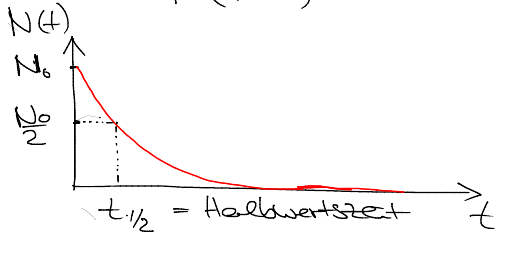
\includegraphics[scale=0.5]{fig6.png}
 \end{figure}

\begin{align*}
  \frac{N_0}{2} &= N_0 \cdot e^{-\lambda t_{\frac 1 2}}\\
  \ln 0.5 &=-\lambda \cdot t_{\frac 1 2} \\
  t_{\frac 1 2} &= - \frac{\ln 0.5}\lambda = {\ln 2}{\lambda} 
\end{align*}

 \begin{ex*}
  \begin{enumerate}[a)]
   \item $\ce{^{224}_{88} Tn} \rightarrow \ce{^{220}_{86} Ru} + \alpha, \qquad \alpha=\ce{^4_2 He}$ mit Halbwertszeit $t_{\frac 1 2}=556s$
   \item $\beta$-Zerfall: $\ce{^{14}_6 C} \to \ce{^{14}_7 N} + e^- \bar v_l$ mit Halbwertszeit $t_{\frac 1 2}=5730 a$  
 \end{enumerate}
 \end{ex*}
 
 
\item Radio-Carbon-Methode \\
 Kohlenstoff: $\ce{^{12}_6 C}, \ce{^{13}_6 C}, \ce{^{14}_6 C}$

 Verteilung in Atmosphäre

 \begin{align*}
  \ce{^{12} C}:  98,89\% \\
  \ce{^{13} C}: 1,11\% \\
 \ce{^{14} C}: 10^-10 \% \\
 \end{align*}
 Wobei erstere beiden stabil und $\ce{^{14} C}$ instabil ist.  Lebende Organismen besitzen aufgrund von Stoffaustausch identische Kohlenstoff-Verteilung.  Stirbt der Organismus verändert sich das Isotopenverhältnis.

 
 \begin{align*}
  \ce{^{14} C(t)}&=\ce{^{14} C_0} \cdot e^{-\lambda t} \\
 \ce{^{13} C(t)}&=\ce{^{12} C_0}\\
 \frac{\ce{^{14} C}}{\ce{^{12} C}} |_\text{Fossil} (t)&= \frac{\ce{^{14} C_0}}{\ce{^{12} C_0}} e^{-\lambda t}, \qquad \lambda=1.121\cdot 10^{-4} \frac{1}{a}
 \end{align*}
 \item C14-Methode: experimentelle Bestimmung\\
 $\frac{\ce{^{14}  C}}{\ce{^{12} C}}$ im Fossil (Massenspektrum) $\rightarrow$ Alter $t \rightarrow$ Alter + Höhlenzeichnung in S-Frankreich:  $15.500$ Jahre
 \end{itemize} 
 \item Länge

 1799: $1 \m \hat = \frac{1}{400000000}$ des durch Paris gehenden Großkreises ($40\cdot 10^3$ km). Dadurch ergab sich die Grundeinheit $1$m.

 Urmeter: $\ce{Pt_{90}}$ $\ce{Ir_{10}}$

 Seit 1983:
 \[
  1\m=\text{ Länge des Weges Weges, den Licht im Vakuum in $\frac{1}{299792485} s$ zurücklegt.}
 \]

\begin{seg}{Größenordnungen und Längen}


 \begin{tabular}{l r}
  Fixstern & $4\cdot 10^16 \m$\\
  Erde-Sonne & $1.5 \cdot 10^11 \m$\\
 Erdradius & $63 \cdot 10^6 \m $\\
 Sichtbares Licht (Wellenlänge) & $ 500\cdot 10^-9$m \\
 Atomdurchmesser & $10^-10$m  \\
 Kerndurchmesser & $10 ^-15$m
 \end{tabular}
 \end{seg}
 \begin{seg}{Messung von Abständen}
 Triangulation:
 \begin{figure}[h]
  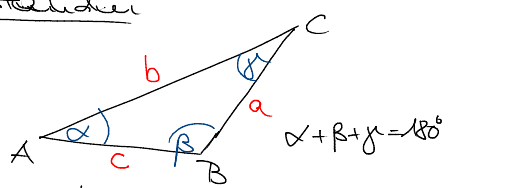
\includegraphics[scale=0.5]{fig7.png}
 \end{figure}
 Sinussatz: $\frac{c}{\sin\gamma} = \frac{a}{\sin{\beta}}=\frac{a}{\sin\alpha}$ \\
 
 \begin{itemize}
  \item $\alpha, \beta$ bekannt $\to \gamma$ bekannt
  \item $c$ bekannt, dann lässt sich $a$ bzw. $b$ berechnen zu:
\begin{align*}
a&=c\cdot \frac{\sin \alpha}{\sin \gamma}\\
b&=c\cdot \frac{\sin \beta}{\sin \gamma}
\end{align*}
 \end{itemize}
\end{seg}
 \begin{seg}{Abstand-Erde-Mond}
 \begin{figure}[h]
  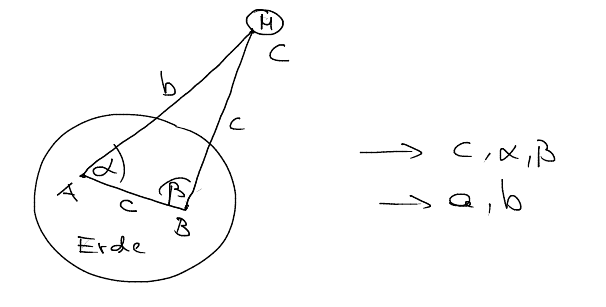
\includegraphics[scale=0.5]{fig8.png}
 \end{figure}
\end{seg}
 \begin{seg}{Abstand Erde-Sonne}
 Als Basis (c) wähle Erde-Mond
 \begin{figure}[h]
  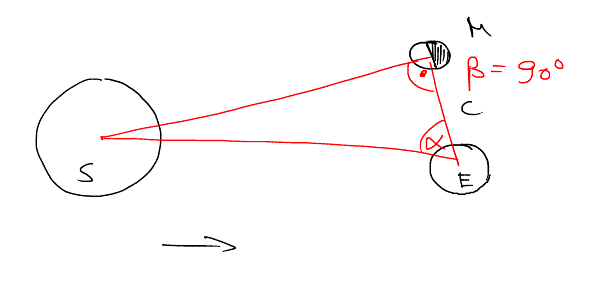
\includegraphics[scale=0.5]{fig9.png}
 \end{figure}
 Bei Halbmond besitzt $\beta=90^\circ$.  Den Abstand Erde-Mond lässt sich messen. Dann genügt es Den Winkel zwischen Mond und Sonne auf der Erde messen und damit ergibt sich der Abstand zum Mond.
 \end{seg}
 \begin{seg}{LIDAR (Light Detection and raging)}
 \begin{figure}[h]
  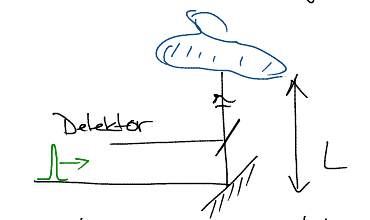
\includegraphics{fig10.png}
 \end{figure}
 \[
 T=\frac{2L}{c}
 \]
\end{seg}
 \begin{seg}{Messungen kleiner Entfernungen Laserinterferometer (\emph{Michelson-Interferometer})}

 \begin{figure}[h]
  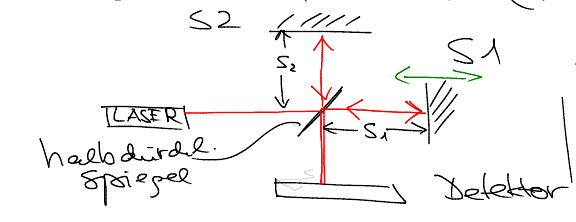
\includegraphics[scale=0.7]{fig11.png}
 \end{figure}

 \[
  \Delta s= 2 |s_1-s_2|
 \]

 Die Verschiebung um $\frac{20 \my m}{\text{64 Maxima}}=0.625 \to \lambda=630\my \m $
\end{seg}
 \item Masse \\
 Die Grundeinheit ist $1kg \hat = \text{Masse des Urkilogramms Zylinder/ } \ce{Pt_{90}}\ce{Ti_{10}}$

 Vermutlich 2014:

 \[
  1 \txt{Mol}= 6022\cdot 10^{23} \cdot \ce{^{28} Si} \hat = 28.09 g
 \]
 \[
 35,599 \,\text{Mol}\, \ce{^{28} Cr} \hat = 1 \kg
 \]
 \[
 2,1441 \cdot 10^{25} \ce{^{28} Si} \text{Atome} \hat = 1 \kg
 \]

 Zeit, Länge, Masse sind die Grundgrößen der Kinematik, die zugehörigen Standardeinheiten bilden das \emph{SI}.
\end{enumerate}
\subsection{Messfehler}
\begin{enumerate}[a)]
\item Systematische Messfehler
\begin{itemize}
\item falsch geeichtes Messinstrument
\item Nichtberücksichtigen von \emph{Konstanten} äußerer Einflüsse
\item Näherungsformeln außerhalb Gültigkeitsbereich (für kleine Winkel $\alpha$ gilt zum Beispiel $\sin \alpha \approx \alpha$ und $\cos \alpha \approx 1$
\end{itemize}
$\implies$ Systematische Messfehler verfälschen Messergebnis um gleichen Betrag und Richtung \\
$\rightarrow$ sie sind also prinzipiell vermeidbar
\item statistische zufällige Messfehler
\begin{itemize}
\item[$\rightarrow$] Können Messergebnis in beide Richtungen verändern.
\item Beobachter selbst 
\item statistische Änderungen äußerer Einflüsse
\item[$\rightarrow$] Die Messwerte streuen daher um einen bestimmten Wert
\item[$\rightarrow$] nicht vermeidbar aber durch wiederholte Messung verringerbar
\end{itemize} 
\end{enumerate}
\begin{seg}{Bildung des arithmetischen Mittels}
Sei unsere Messreihe $x_1, x_2, x_3, ..., x_n$, wobei $n$ die Zahl unserer Messungen darstellt, so ergibt sich das arithmetische Mittel durch:
\[
\boxed{\bar x = \frac{x_1+x_2+x_3+...+x_n}n=\frac{1}{n} \sum_{i=1}^{n} x_i}
\]
Je mehr Messungen gemacht werden, desto genauer entspricht $\bar x$ dem empirischen Mittelwert.  Die \emph{Standardabweichung} $\sigma$ (\emph{Streuung}) gibt an, wie zuverlässig Einzelmessungen sind.
\begin{figure}[h]
%\includegraphics{fig12.png}
\end{figure}
\[
\boxed{\sigma=\sqrt{\frac 1 {n-1} \sum\limits_{i=1}^n (x_i-\bar x)^2}}
\]
Häufig kommt es zur \emph{Gaußverteilung} der Messwerte: Es ergibt sich die Dichtefunktion:
\[
\boxed{p(x)=\frac{1}{\sqrt{2\pi}\cdot \sigma} \cdot e^{-\frac{(x-\bar x)^2}{2\sigma^2}}}
\]
\begin{figure}[h]
%\includegraphics{fig13.png}
\end{figure}
Als Dichtefunktion besitzt $p$ die Eigenschaft: 
\[
\int\limits_{-\infty}^{+\infty}p(x) dx = 1
\]
Die Wahrscheinlichkeit $P$, das x im Intervall $\bar x \pm \sigma$ streut ist damit. 
\[
\int\limits_{\bar x-\sigma}^{\bar x+\sigma} p(x)=0,683
\]
Man bezeichnet dies auch als \emph{statistische Sicherheit} bzw. \emph{Vertrauensgrenze} $P$ für $\delta=\sigma$.

\begin{seg}{Statistische Sicherheit bzw. Vertrauengrenze $P$ für $\delta$}
\begin{table}[h]
\begin{tabular}{c|c}
$\delta[\sigma]$ & $P=\int\limits_{\bar x-\delta}^{\bar x+\delta} p(x) dx$ \\ \hline
1 & 0,683 \\
0,676 & 0,5 \\
1,96 & 0,95 \\
3,0 & 0,997
\end{tabular}
\end{table}
\end{seg}
\end{seg}
\section{Kinematik}
\subsection{Eindimensionale Bewegung}
\begin{enumerate}[a)]
\item gleichförmige Bewegung ($\vec v=\text{const.}$)

\begin{seg}{Weg-Zeit-Diagramm für $\vec v=6\frac{\m}{\s}$}
\begin{figure}[h]
%\includegraphics{fig14.png}
\end{figure}
\end{seg}
Es gilt:
\[
\boxed{\vec v=\frac{\Delta s}{\Delta t} \left (\frac{\m}{\s}\right )}
\]
$\vec v$ ist die Steigung des Weg-Zeit-Diagramms.
\item Nicht-Gleichförmige Bewegung ($\vec v\neq \txt{const.}$)
\begin{figure}[h]
%\includegraphics{fig15.png}
\end{figure}
Die \emph{mittlere Geschwindigkeit} ergibt sich zu:
\[\boxed{\bar v=\frac{\Delta s}{\Delta t}}\]
Die \emph{Momentangeschwindigkeit} entspricht:
\[\boxed{\vec v=\lim\limits_{\Delta t \rightarrow 0} \frac{\Delta s}{\Delta t}= \frac{ds}{dt}}\]
Die Momentangeschwindigkeit $\vec v$ entspricht also der Steigung der Tangente zum Zeitpunkt $t=t_0$. Ist Die Momentangeschwindigkeit nicht konstant, so handelt es sich um eine \emph{beschleunigte} Bewegung.  Die \emph{Beschleunigung} ist für konstante Beschleunigungen gegeben durch:
\[
\boxed{a=\frac{\Delta v}{\Delta t}}
\] 
$a=\txt{const.}$:
\begin{figure}[h]
%\includegraphics{fig16.png}
\end{figure}
$a\neq\txt{const.}$:
\begin{figure}[h]
%\includegraphics{fig17.png}
\end{figure}

Die \emph{Momentanbeschleunigung} ergibt sich zu:
\[
\boxed{a(t)=\lim\limits_{\Delta t \rightarrow 0} \frac{\Delta v}{\Delta t}=\frac{dv}{dt}=\frac{d^2s}{dt^2}\left [\frac{\m}{\s^2}\right ]}
\]
\begin{seg}{Bestimmung von $v(t)$ und $s(t)$}
Es gilt $\frac{dv(t)}{dt}=a(t)$.  Nach integrieren der Gleichung ergibt sich:
\[
\int\limits_0^t \frac{dv(t')}{dt'}dt'=v(t)-v_0=\int\limits_0^t a(t')dt'
\]
wobei $v_0:=v(0)$.  Für $a(t)=a_0=\txt{const.}$ ergibt sich:
\[
\boxed{v(t)=a_0\cdot t+v_0}
\]
Es ist $\frac{ds}{dt}=v$ und es ergibt sich analog:
\begin{align*}
s(t)-s_0&=\int\limits_0^t v(t')dt', s_0:= s(0)\\
s(t)    &=\int\limits_0^t (a_0\cdot t'+v_0)dt'+s_0
\end{align*}
und letztlich ergibt sich:
\[
\boxed{s(t)=\frac{1}{2}a_0t^2+v_0t+s_0}
\]
\end{seg}
\begin{seg}{graphische Darstellung}
\begin{figure}[h]
%\includegraphics{fig18.png}
\end{figure}
Wir können den Weg aus der Beschleunigung bestimmen:
\[
\iint a \,dt\, dt\stackrel{a\approx a_0}{=}\int a_0\cdot t \,dt=\frac{1}{2}a_0t^2=s
\]
\end{seg}
\end{enumerate}
\subsection{Räumliche Bewegung}
Wir können einen Übergang zu vektoriellen Größen Herstellen.  
\begin{figure}[h]
%\includegraphics{fig19.png}
\end{figure}
Wir bezeichnen $\vec r$ als \emph{Ortsvektor} von $P$.  Der Betrag des Vektors ist gegeben durch: $|\vec r|=\sqrt{x_0^2+y_0^2}$.
Wir benutzen die Schreibweise $\vec r=(x_0,y_0)$.  Mögliche Notationen zur Darstellung von Vektoren sind: $\vec r, \stackrel\rightharpoonup r, \underline{r}$.  Für 3-dimensionale Vektoren verwenden wir die Darstellung \[\vec r=\begin{pmatrix} r_x\\ r_y\\r_z \end{pmatrix}; \vec r= \begin{pmatrix} x\\ y\\z \end{pmatrix}\]
\begin{seg}{Addition von Vektoren}
Wir addieren Vektoren komponentenweise:
\[
\vec a+ \vec b=\begin{pmatrix} a_x+b_x\\ a_y+b_y\\a_z+b_z \end{pmatrix}
\]
\begin{figure}[h]
%\includegraphics{fig19.png}
\end{figure}
\end{seg}
\begin{seg}{Subtraktion von Vektoren}
Wir subtrahieren Vektoren komponentenweise:
\[
\vec a- \vec b=\begin{pmatrix} a_x-b_x\\ a_y-b_y\\a_z-b_z \end{pmatrix}
\]
\begin{figure}[h]
%\includegraphics{fig20.png}
\end{figure}
Beschreibung von Vektoren ist abhängig vom Koordinatensystem:
\end{seg}

\begin{seg}{Kartesisches Koordinatensystem (rechtwinklig, rechtshändig}
\begin{figure}[h]
%\includegraphics{fig21.png}
\end{figure}[h]
\begin{figure}[h]
%\includegraphics{fig22.png}
\end{figure}
$r(t)$ ist ein zeitabhängiger Ortsvektor und beschreibt dadurch eine Ortskurve. Die Notation:
\[
\vec r(t)=\begin{pmatrix} x(t)\\ y(t)\\z(t) \end{pmatrix}
\]
Alternativ ist auch denkbar:
\begin{align*}
\vec r(t)&=(x(t),y(t),z(t))\\
\vec r(t)&=x(t)\cdot \vec e_x+y(t)\cdot \vec e_y+z(t)\cdot\vec e_z
\end{align*}
wobei $\vec e_x, \vec e_y, \vec e_z$ die Einheitsvektoren der Koordinatenachsen sind. Der Betrag des Vektor ergibt sich zu:
\[
r(t)=|\vec r|=\sqrt{{x(t)}^2+{y(t)}^2+{z(t)}^2}
\]
\end{seg}
Wir erinnern uns an die Definition für die Geschwindigkeit für eindimensionale Bewegungen:
\begin{align*}
v&=\frac{ds}{dt}\\
a&= \frac{dv}{dt}=\frac{d^2s}{dt^2}
\end{align*}
f+r $a=a_0=\txt{const.}$ ergab sich:
\begin{align*}
v(t)&=a_0\cdot t+v_0, v_0=v(0)\\
s(t)&= \frac{1}{2} a_0t^2+v_0\cdot t+s_0, s_0=s(0)
\end{align*}
Betrachten wir also eine Bewegung, die durch eine Ortskurve gegeben ist.
\begin{figure}[h]
%\includegraphics{fig23.png}
\end{figure}
Sei $\Delta r=r(t+\Delta t)-r(t)$ Für $\Delta t\rightarrow 0$ gilt $\Delta s\approx \Delta r$.  Folgende Definitionen für Geschwindigkeit und Beschleunigung sind daher naheliegend:
\begin{df}[Geschwindigkeit]
Die Geschwindigkeit $\vec v(t)$ ist definiert durch:
\[\vec v(t)=\lim\limits_{\Delta t\rightarrow 0} \frac{\Delta \vec r}{\Delta t} = \frac{d\vec{r}}{dt}=\dot{\vec r}=(\frac{dx}{dt},\frac{dy}{dt},\frac{dz}{dt})=(v_x(t),v_y(t),v_z(t))\]
Hierbei zeigt $\vec v(t)$ in Richtung der Bahntangente an die Ortskurve $\vec r(t)$.
\end{df}
\begin{df}[Beschleunigung]
Die Beschleunigung $\vec v(t)$ ist definiert durch:
\[\vec a(t)=\lim\limits_{\Delta t\rightarrow 0} \frac{\Delta \vec v}{\Delta t} = \frac{d\vec{v}}{dt}=\frac{d^2\vec{v}}{dt^2}=\ddot{\vec r}=(\frac{d^2x}{dt^2},\frac{d^2y}{dt^2},\frac{d^2z}{dt^2})=(a_x(t),a_y(t),a_z(t))\]
\end{df}
Wir betrachten nun die Beschleunigung zur Bahn eines Massenpunkts.  Diese ist im Allgemeinen nicht mit der Bahntangenten identitisch. $\vec a$ kann sowohl eine Tangentialkomponente wie auch eine Normalkomponente besitzen. Wir bezeichnen in Folge den Einheitsvektor tangential zur Bahnkurve mit $\vec u_T$.
\[
\boxed{\vec a=\frac{d\vec{v}}{dt}=\frac{d}{dt}(|\vec v|\cdot \vec u_T)=\underbrace{\frac{d|\vec v|}{dt}\cdot\vec u_T}_{\txt{\tiny{Tangentialkomponente}}}+\underbrace{|\vec v|\cdot \frac{d\vec{u_T}}{dt}}_{\txt{\tiny{Normalkomponente}}}} 
\]
\begin{enumerate}
\item geradlinige Bahn des Massenpunktes
\begin{figure}[h]
%\includegraphics{fig24.png}
\end{figure}
$\vec u_T$ zeigt immer in gleiche Richtung und damit ist $\frac{d\vec{u_T}}{dt}=0$ und
\[
\boxed{\vec a=\frac{d|\vec v|}{dt}\cdot {\vec{u_T}}}
\]
$\vec v$ und $\vec a$ besitzen gleiche Richtung.
\item betrachten wir eine gekrümmte Bahn so ist $\frac{d\vec{u_T}}{dt}\neq 0$
\begin{figure}[h]
%\includegraphics{fig25.png}
\end{figure}
Unter Ausnützung der Ähnlichkeit der beiden Dreiecke ergibt sich bei einer Kreisbahn gerade:
\[
\frac{|\Delta \vec u_T|}{|\vec u_T|}=\frac{\Delta s}{R}\implies |\Delta \vec u_T|=\frac{1}{R}\cdot \Delta s
\]
nach dem Differenzieren auf beiden Seiten (Überlegen Sie sich, warum sie dies so machen dürfen!):
\[
|\frac{d\vec{u_T}}{dt}|=\frac{1}{R}\cdot |\vec v|
\]
Die Normalkomponente steht dabei gerade orthogonal zum Tangentialkomponente der Beschleunigung (Übung!), denn es gilt $\frac{d\vec{u_T}}{dt}\perp   \vec u_T$ (Übung!), dies ist gerade dann der Fall, wenn $\alpha \rightarrow 0$. Man sagt $\frac{d\vec{u_T}}{dt}$ steht "`normal"' zur Bahnkurve.
\begin{figure}[h]
%\includegraphics{fig26.png}
\end{figure}
Es ergibt sich für die Beschleunigung:
\[
\va=\frac{d|\v|}{dt} \cdot \u_T+\vec{u_N}\cdot \frac{d\u_T}{dt}=\underbrace{\frac{d|\v|}{dt}}_{a_T} \cdot \u_T+\underbrace{\frac{|\v|^2}{R}}_{a_N}\cdot \vec{u_N}
\]
Der Betrag von $\va$ ergibt sich zu: $|\va|=\sqrt{a_T^2+a_N^2}=\sqrt{\left (\frac{d|\v|}{dt}\right )^2+\left ( \frac{v^2}R \right )^2}$
\end{enumerate}
\begin{ex*} Wir betrachten zwei Spezialfälle
\begin{enumerate}[a)]
\item geradlinige Bewegung
\[
R\rightarrow \infty \implies a_N\rightarrow 0
\] 
\item $|\v|=\txt{const.} \implies a_T=0$, aber $a_N\neq 0$. Es handelt sich hierbei um eine Kreisbewegung. 
\end{enumerate}
\end{ex*}
Es gilt das \emph{Superpositionsprinzip:}

\begin{seg}{Superpositionsprinzip:} Wenn ein Körper mehrere Bewegungen in verschiedenen Richtungen gleichzeitig ausführt, dann sind die Bewegungen in jeder Richtung unabhängig von den Bewegungen in den anderen Richtungen. 
\end{seg}
\begin{seg}{lineare Überlagerung von Bewegun in unterschiedliche Raumrichtungen}
\begin{itemize}
\item \emph{horizontaler Wurf}\\
Beim horizontalen Wurf komm es zu einer Überlagerung von konstanter horizontaler Geschwindigkeit $v_{x_0}$ und freien Fall.
\begin{align*}
x&=v_{x_0}\cdot t\\
y&=-\frac 1 2 \underbrace{g}_{\approx 10\frac{\m}{\s^2}}t^2
\end{align*}
\begin{figure}[h]
%\includegraphics{fig27.png}
\end{figure}
\[
t=\frac{x}{v_{x_0}} \implies \boxed{y=-\frac{1}{2} g \frac{x^2}{v_{x_0}^2}}
\]
Damit besitzt die Ortskurve eine Parabelbahn. Ihr Maximum nimmt sie gerade im Ursprung an.
\item \emph{Schiefer Wurf}\\
Beim schiefen Wurf kommt es zur Überlagerung von konstanter Geschwindigkeit in beliebiger Richtung und dem freien Fall. Zunächst lässt sich $\vec v_0$ in Horizontal- und Vertikalkomponente aufspalten:
\[
\v_0=\v_{0x}+\v_{0y}
\]
Für die Komponenten ergibt sich in Abhängigkeit zur Zeit $t$:
\begin{align*}
x&=v_{x_0}\cdot t\\
y&=v_{y_0}\cdot t-\frac{1}{2}gt^2
\end{align*}
\begin{figure}[h]
%\includegraphics{fig28.png}
\end{figure}
Es ergibt sich die Parabelbahn:
\[
\boxed{y=v_{y_0}\cdot \frac{x}{v_{x_0}}-\frac 1 2 g \frac{x^2}{v_{x_0}^2}}
\]
\item \emph{Kreisbewegung}\\
Bei der Kreisbewegung gilt:
\begin{align*}
x&=R\cdot\cos{\phi}\\
y&=R\cdot\sin{\phi}
\end{align*}
Für $\frac{d\phi}{dt}=\txt{const.}$ ergibt sich eine gleichförmige Kreisbewegung, der Betrag der Geschwindigkeit ist konstant.  
\begin{df}[Winkelgeschwindigkeit]
Die Winkelgeschwindigkeit $\omega$ ist definiert durch:
\[
\omega =\frac{d\phi}{dt}
\]
Entsprechend gilt $v=\frac{ds}{dt}$.
\end{df}
Die Einheit von $\omega$ ist $\frac{\txt{rad}}{\s}$ bzw. $\frac 1 \s$
\end{itemize}
\begin{seg}{Exkurs: Winkelmessung}
Es gibt zwei Möglichkeiten Winkelgrößen zu definieren, entweder in dem man $1$° als Teil eines Vollkreises.
\[
1^\circ \hat = \frac{1}{360} \txt{Vollkreis}
\]
oder über die Bogenlänge am Einheitskreis (also als \emph{Radiant}). Charakteristische Größen sind:
\begin{align*}
360°&=2\pi=6,28 \rad\\
1 \rad &\approx 57,29°\\
1°&\approx 0,0017 \rad
\end{align*}
$\rad$ ist eine dimensionslose Größe.
\end{seg}
$\omega$ ist ein Vektor mit Betrag $|\omega|=\frac{d\phi}{dt}$ orthogonal zur Kreisebene gerichtet.
\begin{figure}[h]
%\includegraphics{fig29.png}
\end{figure}
Die Richtung von $\omega$ bestimmt sich mittels der \emph{rechte-Hand-Regel}:
\begin{figure}[h]
%\includegraphics{fig30.png}
\end{figure}
Für den Winkel gilt also bei einer gleichförmigen Kreisbewegung:
\[
\phi(t)=\omega\cdot t
\]
bzw. für die Komponenten:
\begin{align*}
x&=R\cdot \cos(\omega t)\\
y&=R\cdot \sin(\omega t)
\end{align*}
Für die \emph{Periodendauer} $T$ (Zeit für einen Umlauf) ergibt sich $T=\frac{2\pi}{\omega}$. Für die \emph{Frequenz} $\nu$ (Zahl der Umläufe pro Sekunde) ergibt sich $\nu=\frac{1}{T}=\frac{\w}{2\pi}$. Die Geschwindigkeit des Massenpunktes P auf der Kreisbahn ist bestimmt zu $|\v|=\frac{2\pi\cdot R}{T} \hat=\frac{\txt{Strecke}}{\txt{Umlaufzeit}}$ und damit $|\v|=\omega \cdot R$.

Für $\omega=\txt{const.}$ ist auch $|v|=\const$, aber die Richtung von $\vec v$ ändert sich, da sie tangential zur Bahnkurve gerichtet ist. 
\end{seg}

\end{document}
